\documentclass[twoside,twocolumn]{article}
    \usepackage[a4paper, left=2cm, right=2cm]{geometry} % A4 paper size and thin margins
    \usepackage[sc]{mathpazo} % Use the Palatino font
    \usepackage[T1]{fontenc} % Use 8-bit encoding that has 256 glyphs
    \usepackage{microtype} % Slightly tweak font spacing for aesthetics
    \usepackage[english]{babel} % Language hyphenation and typographical rules
    \usepackage{booktabs} % Horizontal rules in tables
    \usepackage{lettrine} % The lettrine is the first enlarged letter at the beginning of the text
    \usepackage{enumitem} % Customized lists
    \usepackage{xcolor} % Required for specifying custom colours
    \usepackage[utf8]{inputenc} % Required for inputting international characters
    \usepackage{parskip}
    \usepackage{graphicx}
    \usepackage{hyperref}
    \usepackage{pdfpages}
    \usepackage[title]{appendix}
    \hypersetup{
        colorlinks=true,
        linkcolor=blue,
        filecolor=magenta,      
        urlcolor=cyan,
    }
    \urlstyle{same}
    \setlength{\parindent}{15pt}
    \setlist[itemize]{noitemsep} % Make itemize lists more compact
    \definecolor{grey}{rgb}{0.9,0.9,0.9} % Colour of the box surrounding the title
    \makeatletter
    \newcommand*{\rom}[1]{\expandafter\@slowromancap\romannumeral #1@}
    \g@addto@macro{\UrlBreaks}{\UrlOrds}
    \makeatother

    %----------------------------------------------------------------------------------------
    %	TITLE PAGE
    %----------------------------------------------------------------------------------------
    \begin{document}
    \begin{titlepage}
        
        %------------------------------------------------
        %	Title box
        %------------------------------------------------
        
        \colorbox{grey}{
            \parbox[t]{0.93\textwidth}{ % Outer full width box
                \parbox[t]{0.91\textwidth}{ % Inner box for inner right text margin
                    \raggedleft % Right align the text
                    \fontsize{40pt}{80pt}\selectfont % Title font size, the first argument is the font size and the second is the line spacing, adjust depending on title length
                    \vspace{0.7cm} % Space between the start of the title and the top of the grey box
                    Distinguishing\\
                    News From\\
                    Fake News\\
                    \vspace{0.7cm} % Space between the end of the title and the bottom of the grey box
                }
            }
        }
        
        \vfill % Space between the title box and author information
        
        %------------------------------------------------
        %	Author name and information
        %------------------------------------------------
        
        \parbox[t]{0.93\textwidth}{ % Box to inset this section slightly
            \raggedleft % Right align the text
            \large % Increase the font size
            {\Large Chongyi Xu}\\[4pt] % Extra space after name
            CSE 415, Fall 2017\\
            Assignment 7 Report\\
            Univerisity of Washington\\[4pt] % Extra space before URL
            
            \hfill\rule{0.2\linewidth}{1pt}% Horizontal line, first argument width, second thickness
        }
        
    \end{titlepage}

    %----------------------------------------------------------------------------------------
    %	ARTICLE CONTENTS
    %----------------------------------------------------------------------------------------

    \linespread{1.05} % Line spacing - Palatino needs more space between lines
    %------------------------------------------------
    \section{Introduction}

    \subsection{Definition}
    Fake news problem refers to fabricated news or plain 
    government propaganda with huge ramifications in the current society. In general, 
    fake news is explained in 7 types of fake content according to First Draft News, 
    the organization dedicated to improving skills and standards in the reporting and 
    sharing of online information. False connection, false context, manipulated content,
    satire or parody, misleading content, imposter content, and fabricated content.

    \subsection{History}
    In 19th century, one example of the fake news the 
    \emph{Greate Moon Hoax} of 1835. The New York Sun published articles about a real-life 
    astronomer and a made-up colleague who, according to the hoax, had observed bizarre 
    life on the moon. The fictionalized articles successfully attracted new subscribers, 
    and the penny paper suffered very little backlash after it admitted the next month 
    that the series had been a hoax. Such stories were intended to entertain readers, and 
    not to mislead them. \\20th century during WW\rom{1}, one of the most notorious fake news
    was that of an alleged German Corpse Factory in which the German battlefield dead were 
    rendered down for fats used to make nitroglycerine, candles, lubricants, human soap, and
    boot dubbing.Unfounded rumors regarding such a factory circulated in the Allied press 
    starting in 1915, and by 1917 the English-language publication North China Daily News 
    presented these allegations as true at a time when Britain was trying to convince China 
    to join the Allied war effort; this was based on new, allegedly true stories from The 
    Times and The Daily Mail that turned out to be forgeries. These false allegations became 
    known as such after the war, and in the Second World War Joseph Goebbels used the story 
    in order to deny the ongoing massacre of Jews as British propaganda. According to Joachim
     Neander and Randal Marlin, the story also \"encouraged later disbelief\" when reports 
     about the Holocaust surfaced after the liberation of Auschwitz and Dachau concentration 
     camps.
    %------------------------------------------------
    \section{Formulation}
    My problem formulation is identical to George Mclntire's work based on 
    \href{https://opendatascience.com/blog/how-to-build-a-fake-news-classification-model/}{opendatascience}. 
    The data gathering is in two parts. The first part is getting fake news part, which generally 
    focusing on importing the \href{https://www.kaggle.com/mrisdal/fake-news}
    {fake news dataset} from Kaggle with 13,000 articles published during the 2016 election cycle. The second
    part is to get "real" news from \href{https://www.allsides.com/unbiased-balanced-news}{AllSlides}, according to
    \href{https://opendatascience.com/blog/how-to-build-a-fake-news-classification-model/}{George Mclntire's blog},
    he ended up scraping a total of 5279 articles came from media organizations that were published in 2015 or 2016. 
    
    %------------------------------------------------

    \section{Techniques Used}
    I basically chosed 4 classifiers to implement and compare. My purpose is the find the "better" classifier
    for solving Fake News Problems.
    \subsection{Naive Bayes}
    Navice Bayes Classifier is a probabilistic classifier based on applying Bayes' theorm with naive independece
    assumptions. It combines the Bayes' probability model with a decision rule. One common rules is to pick the 
    hypothesis that is most probable; that is known as the maximum a posteriori or MAP decision.
    \\ In this case, I am going to develop a multinomial naive Bayes, where vectors represent the frequencies 
    with which certain events have been generated by a multinomial ($p_{1},\dots ,p_{n}$) where 
    $p_{i}$ is the probability that event $i$ occurs

    \subsection{Support Vector Machine}
    Support Vector Machines (SVMs) are classifiers with associated learning algorithm that analyze data. Given 
    a set of training examples, each marked as belonging to one or the other of two categories, an SVM training 
    algorithm builds a model that assigns new examples to one category or the other, making it a non-probabilistic 
    binary linear classifier.

    \subsection{Differnce \& Similarity}
    Naive Bayes Classifier (NBC) and Support Vector Machine (SVM) have different options including the choice 
    of kernel function for each. They are both sensitive to parameter optimization (i.e. different parameter 
    selection can significantly change their output) . So, if you have a result showing that NBC is performing 
    better than SVM. This is only true for the selected parameters. However, for another parameter selection, 
    you might find SVM is performing better.
    \\In general, if the assumption of independence in NBC is satisfied by the variables of your dataset and the 
    degree of class overlapping is small (i.e. potential linear decision boundary), NBC would be expected to 
    achieve good. For some datasets, with optimization using wrapper feature selection, for example, NBC may 
    defeat other classifiers. Even if it achieves a comparable performance, NBC will be more desirable because 
    of its high speed.

    \subsection{Other Classifiers}
    Besides NBC and SVM, I am also considering other 2 classifiers to compare results.
    \begin{itemize}
        \item Decision Tree
        \item K Nearest Neighbors
    \end{itemize}
    %------------------------------------------------

    \section{Training and Testing Data Used}
    The data I am going to use is from \href{https://s3.amazonaws.com/assets.datacamp.com/blog_assets/fake_or_real_news.csv}
    {datacamp}. The table has the following columns
    \begin{itemize}
        \item \emph{Unnamed: 0:} unique id
        \item \emph{title:} title of an article
        \item \emph{text:} content of an article
        \item \emph{label:} the label telling if the data is fake or real
    \end{itemize}

    \noindent And sample table is like

    \noindent 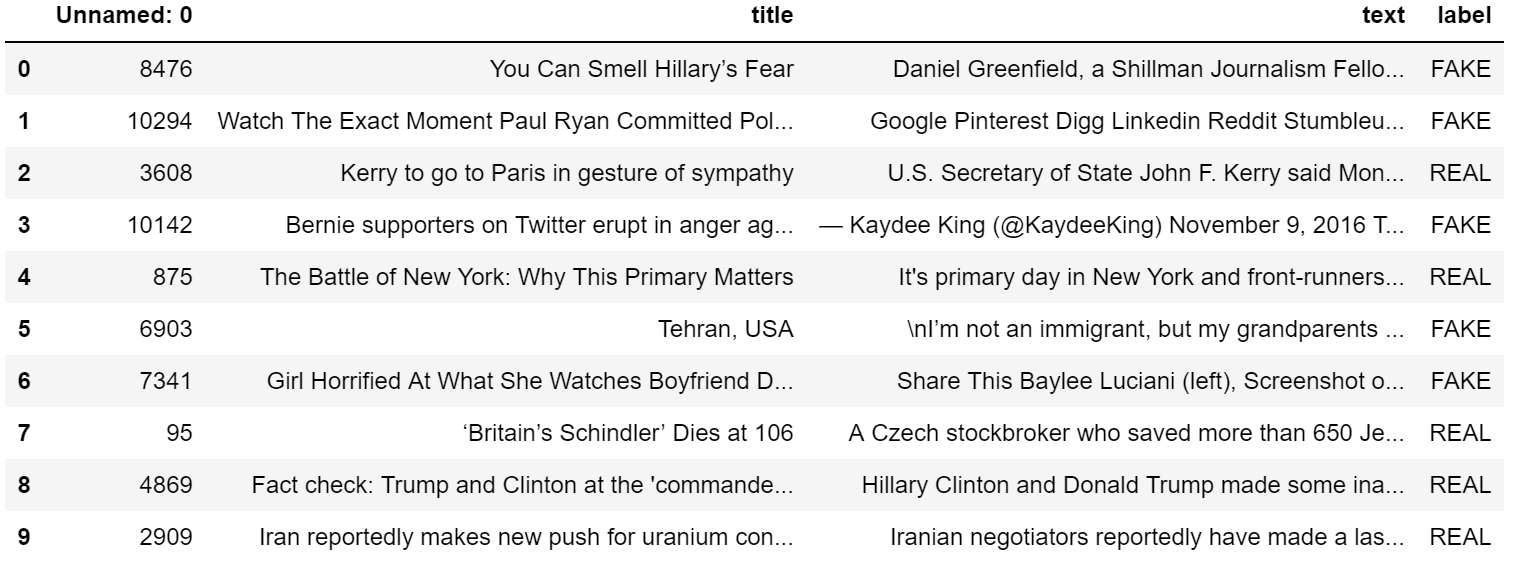
\includegraphics[scale=0.4]{figures/data_table.png}

    \noindent And the dataset has 6335 rows with 4 colunmns.


    \section{Experiments}
    
    \subsection{Seprate Training Data \& Testing Data}
    Since the dataset itself has more than 5000 observations, I decided to seperate
    the set into training set and testing set. The seperation method I am using is randomly pick 1/3 of the 
    data as testing set. In order to keep my training set and testing set consistent every time, I picked a 
    seed number.
    \\ With random seperation, I got two set of tuple data, $(x_train, y_train)$
    and $(x_test, y_test)$ where training set contains 4244 rows and testing set
    contains 2091 rows. Some sample training data is like
    
    \noindent 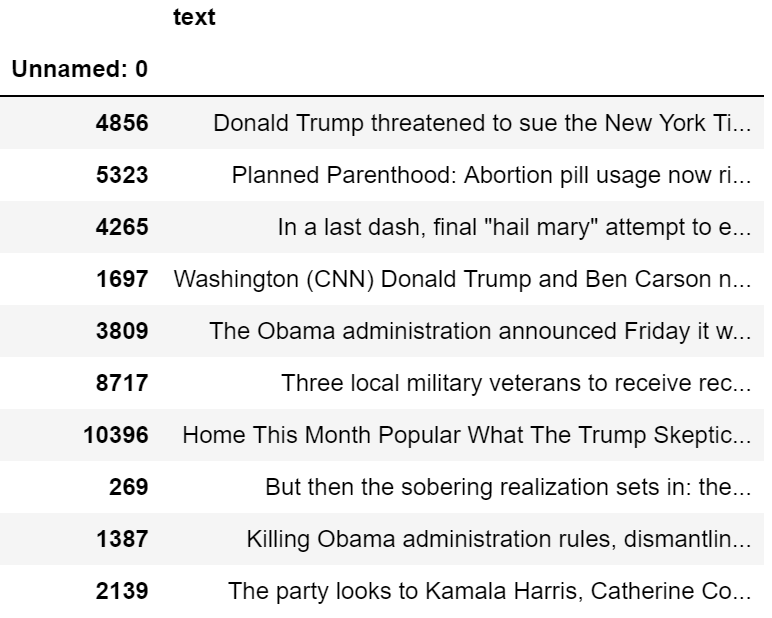
\includegraphics[scale=0.8]{figures/train_data.png}
    
    \noindent And in each dataset,  ~50\% of the news are real and about the 
    other half are fake. And the csv file is 29.2MB which is an ideal input size 
    to run on personal laptop.
    
    \subsection{Vectorize Data}
    In order to apply classifier, it is neccessary to change the data table into vectors.
    \subsubsection{tf-idf}
    TFIDF or tf-idf, short of term frequency-inverse document frequency, is a numerical statistic that reflects
    how important a word is to a document (article) in a collection or corpus.
    \subsubsection{CountVectorizer}
    CountVectorizer counts the word frequencies in the article.

    \section{Results}
    \subsection{Naive Bayes Classifier}
    \subsubsection{CountVectorizer}
    f1 score: 0.89314\\
    \\ \noindent 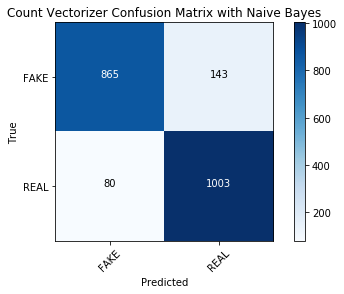
\includegraphics[scale=0.6]{figures/NBC_count.png}
    
    \subsubsection{TFIDF}
    f1 score: 0.85403\\
    \\ \noindent 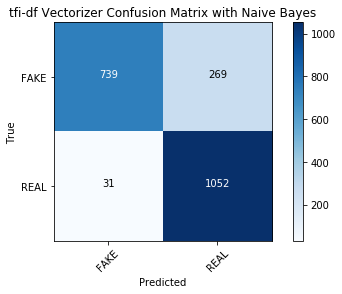
\includegraphics[scale=0.6]{figures/NBC_tfidf.png}
    
    \subsection{Support Vector Machine(SVM)}
    \subsubsection{CountVectorizer}
    f1 score: 0.90722\\
    \\ \noindent 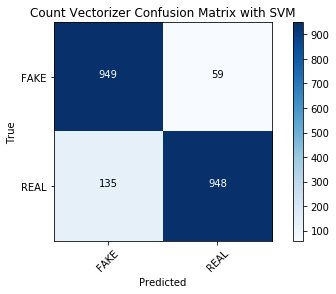
\includegraphics[scale=0.6]{figures/SVM_count.png}
    \subsubsection{TFIDF}
    f1 score: 0.70916\\
    \\ \noindent 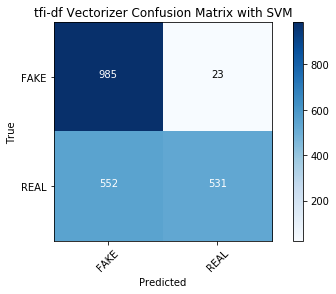
\includegraphics[scale=0.6]{figures/SVM_tfidf.png}
    
    \subsection{Decision Tree}
    \subsubsection{CountVectorizer}
    f1 score: 0.77441\\
    \\ \noindent 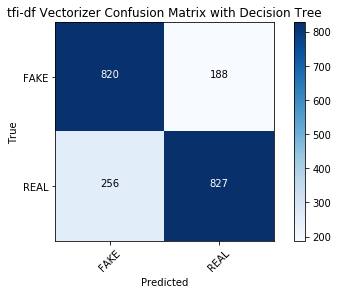
\includegraphics[scale=0.6]{figures/tree_count.png}
    \subsubsection{TFIDF}
    f1 score: 0.78912\\
    \\ \noindent 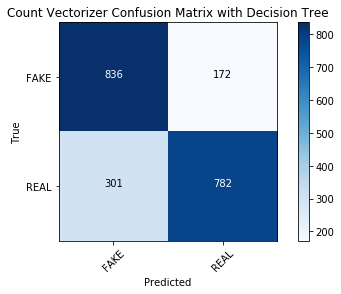
\includegraphics[scale=0.6]{figures/tree_tfidf.png}

    \subsection{KNeighbors Classifier}
    \subsubsection{CountVectorizer}
    f1 score: 0.80385\\
    \\ \noindent 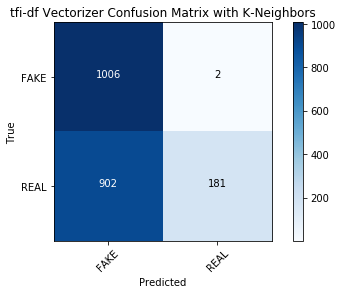
\includegraphics[scale=0.6]{figures/knn_count.png}
    \subsubsection{TFIDF}
    f1 score: 0.48072\\
    \\ \noindent 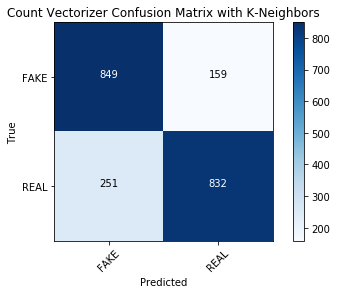
\includegraphics[scale=0.6]{figures/knn_tfidf.png}

    \subsection{Comparison of F1 Scores}
    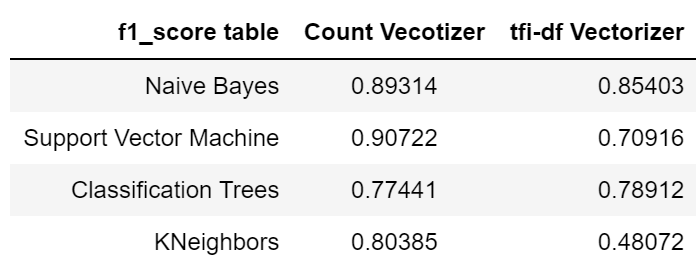
\includegraphics[scale=0.9]{figures/f1.png}
    \section{Discussion}
    Currently, society is suffering "Fake News" among various social media. It is our duty to 
    distinguish those fakes from truth. In the process of formulating the problem, it took me
    a long time to figure out the real news for the import of my training data.
    \\ As a result, I found that generlly, SVM could give a better result on distinguishing fake
    and real news when we vectorize our data considering the appearence of every words. Meanwhile, 
    if we vectorize the text considering the importance of every words in the text content, Naive
    Bayes Classifier might perform better.
    \section{Personal Retrospective}
    In this assignment, I have learned more about the Fake News Problem, such as how important it
    is to the society and the difficulty to solve for it. Fake News could affect a lot to politics,
    natural science, economics and all the way to every single field. I also learned the pros and 
    cons of data analyzing classifiers, for instance, naive Bayes, K Nearest Neighborsr, Decision Tree,
    and Support Vector Machines. It is always a good idea to test all classifiers since we could not 
    be familier to the processing dataset everytime to know which classifier should be used. 
    %----------------------------------------------------------------------------------------
    %	REFERENCE LIST
    %----------------------------------------------------------------------------------------

    \begin{thebibliography}{99} % Bibliography

    \bibitem[1]{1}
    A new database of fake news sites details how much fakery has spread from Trump v. 
    Clinton to local news by LAURA HAZARD OWEN @laurahazardowen April 21, 2017, 10:17 a.m. \url{http://www.niemanlab.org/2017/04/a-new-database-of-fake-news-sites-details-how-much-fakery-has-spread-from-trump-v-clinton-to-local-news/}

    
    \bibitem[2]{2}
    Social Media and Fake News in the 2016 Election Journal of Economic Perspectives—Volume 31, 
    Number 2—Spring 2017—Pages 211–236 \url{https://web.stanford.edu/~gentzkow/research/fakenews.pdf}

    \bibitem[3]{3}
    A comparison of a several classifiers in scikit-learn on synthetic datasets. Illustrating the nature 
    of decision boundaries of different classifiers. \url{http://scikit-learn.org/stable/auto_examples/classification/plot_classifier_comparison.html}
    
    \bibitem[4]{4}
    When does Naive Bayes perform better than SVM? \url{https://stats.stackexchange.com/questions/58214/when-does-naive-bayes-perform-better-than-svm}
    \end{thebibliography}

    %----------------------------------------------------------------------------------------

    %-------------------------------
    % Appendices
    %-------------------------------
    \newpage
    \appendix
    \section{Appendix A}
    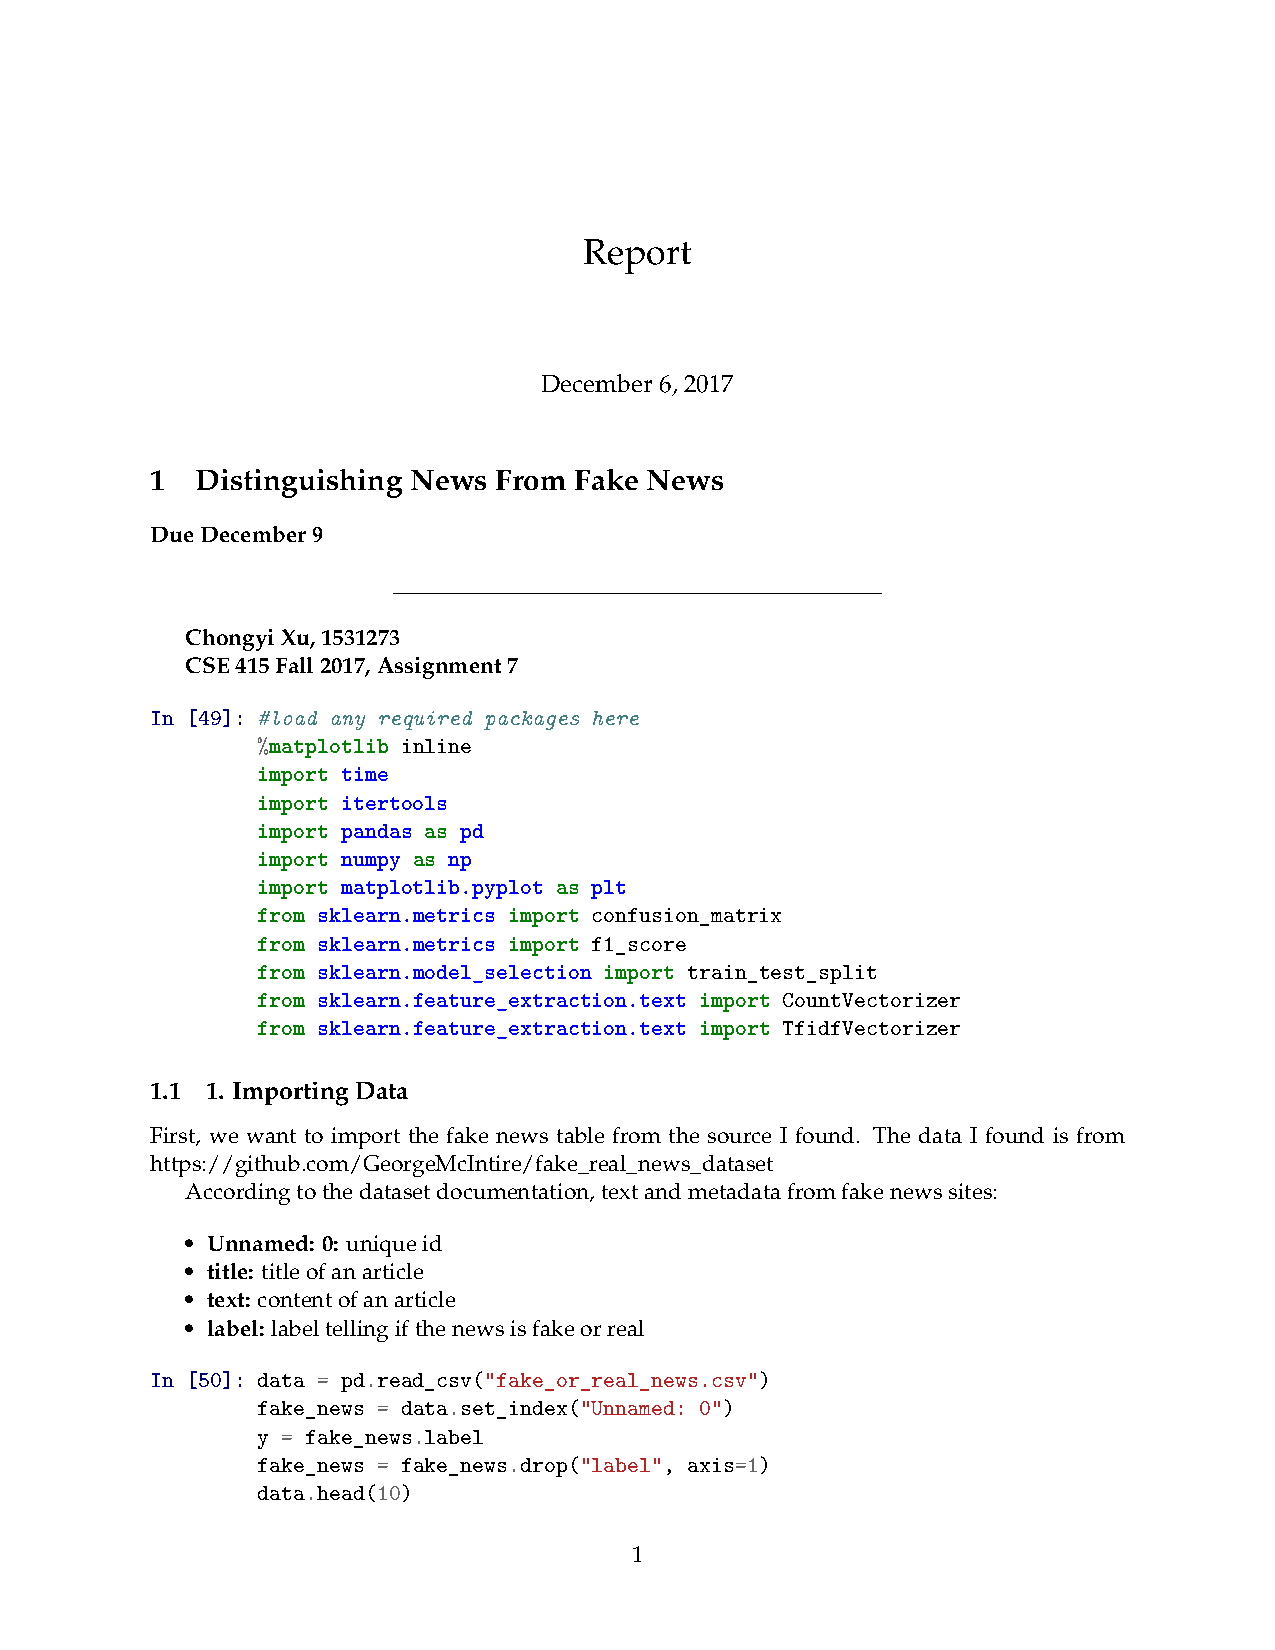
\includepdf[pages=1-11]{jupyter.pdf}
\end{document}